\chapter{Reconciled Framework Architecture}
\label{ch:framework-reconciliation}

\section{Why concatenation is not integration}

The retained framework corpus contains eight text files, but they are not eight
independent theories. A deterministic paragraph audit finds that
\texttt{Alpha001.06} and \texttt{Maximal Extraction} contain the same 390
unique normalized blocks. The former repeats these blocks until 2,078 eligible
block occurrences remain, of which 1,688 are internal duplicates. Counting
these repetitions as agreement would turn copying into evidence.

The consolidation therefore preserves the original documents as archival
sources and constructs a new framework from unique claims. Exact duplicate
spans collapse to one canonical statement with multiple provenance aliases.
Similar headings nominate a semantic review; they do not authorize merging
different equations or physical mechanisms.

\begin{figure}[htbp]
  \centering
  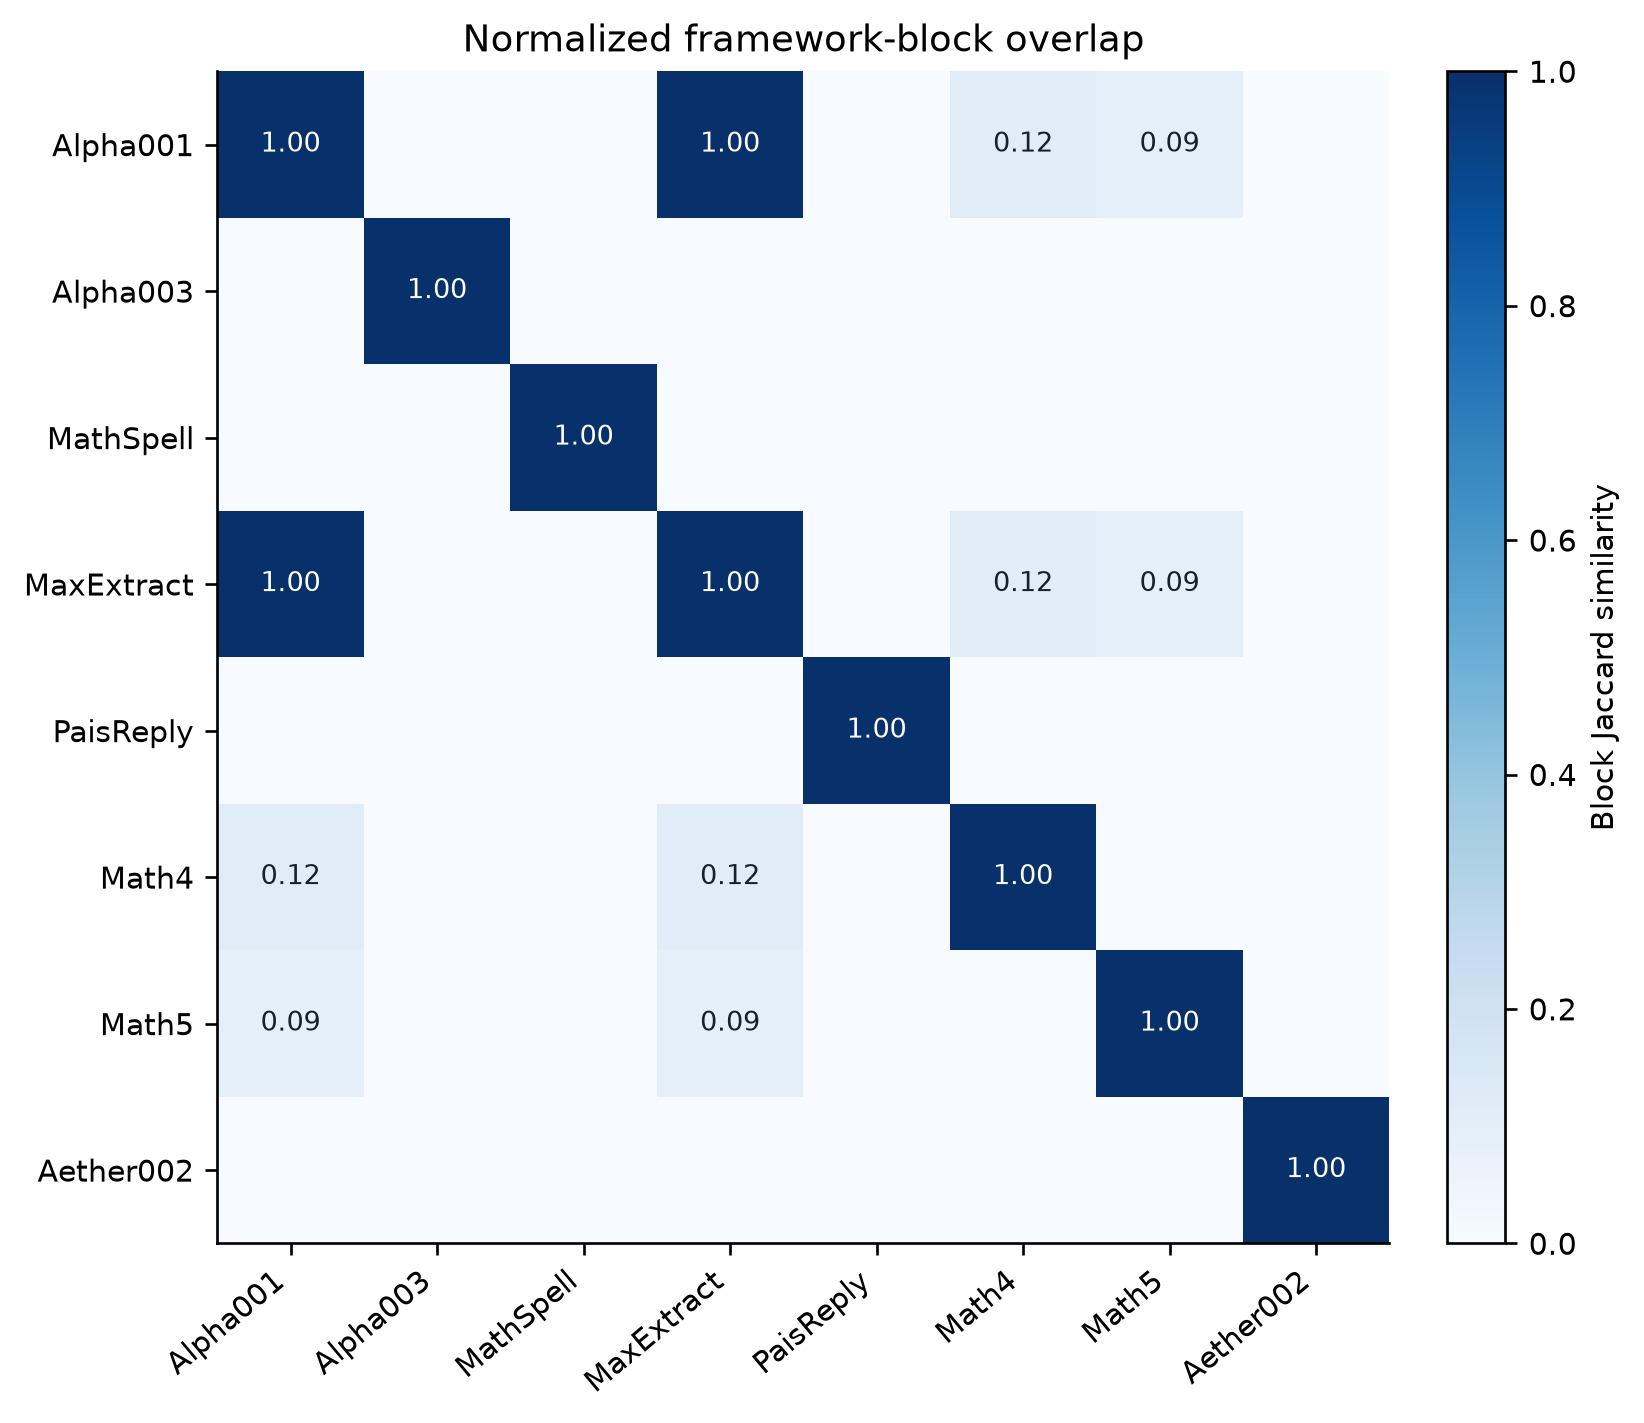
\includegraphics[width=0.82\textwidth]{figures/review_framework_overlap.png}
  \caption{Exact normalized-block overlap among the eight retained framework
  documents. The unit overlap identifies duplicate lineage rather than
  independent corroboration.}
  \label{fig:framework-overlap}
\end{figure}

\section{One framework, five evidence layers}

The unified framework is organized by evidential role rather than source order.

\begin{description}
  \item[Defined mathematics] Octonions, higher Cayley--Dickson algebras,
    exceptional and Kac--Moody algebras, the Albert algebra, lattices, modular
    forms, spectral geometry, and named notions of dimension enter with their
    standard definitions and known boundaries.
  \item[Typed bridges] A cross-domain map must name its source object, target
    object, map, preserved invariants, assumptions, and observable.
  \item[Reproducible computation] Code enters only after schema, determinism,
    invariant, refinement, and control gates appropriate to its claim.
  \item[Physical hypotheses] A proposed mechanism must descend from a defined
    action, Hamiltonian, constitutive law, or stochastic process and must state
    units, parameters, observables, and a null model.
  \item[Historical ideation] Undefined analogies and nonempirical claims remain
    traceable but do not enter the scientific core.
\end{description}

This architecture preserves productive conjectures without allowing them to
inherit theorem-level confidence from the mathematical objects they mention.

\section{Resolved mathematical conflicts}

\subsection{Cayley--Dickson scope}

The real normed division algebras stop at the octonions
\citep{baez2001octonions}. Higher Cayley--Dickson doublings remain legitimate
algebraic objects, and their zero divisors are mathematically structured
\citep{moreno2005constructing}; however, division, norm composition, and other
identities cannot be assumed to persist. A proposed physical application must
identify the exact multiplication law, subspace, invariant, and observable it
uses. Dimension alone supplies no mechanism.

\subsection{Albert algebra and exceptional groups}

The source statement that $E_6$ is the automorphism group of
$J_3(\mathbb{O})$ and $E_7$ the automorphism group of a sedenionic
$J_3(\mathbb{S})$ is rejected. The Albert algebra is built from octonions;
$F_4$ is its automorphism group, while suitable forms of $E_6$ and $E_7$ arise
as structure and conformal groups \citep{baez2001octonions}. These group
actions are different objects,
not interchangeable meanings of \enquote{symmetry}.

\subsection{The E-series boundary}

$E_6$, $E_7$, and $E_8$ are finite-dimensional exceptional simple Lie
algebras. $E_9$, $E_{10}$, and $E_{11}$ are affine, hyperbolic, and
very-extended Kac--Moody structures. Restricted supergravity dictionaries
motivate research programs \citep{damour2002e10,west2001e11}; they do not prove
a complete symmetry of observed interactions.

\section{Resolved physical boundaries}

\subsection{Time crystals}

The equilibrium continuous-time-crystal proposal is excluded under broad
conditions by the Watanabe--Oshikawa no-go theorem
\citep{watanabe2015absence}. Floquet time crystals are instead driven
nonequilibrium many-body phases \citep{else2016floquet}, and primary experiments
observe their subharmonic response \citep{zhang2017observation}. The drive,
dissipation, and finite lifetime remain part of the energy budget. These results
do not supply free amplification of vacuum energy.

\subsection{Vacuum response and energy extraction}

Casimir forces do not by themselves prove that zero-point energy is an
extractable reservoir \citep{jaffe2005casimir}. Dynamical-Casimir photon
production uses work supplied through a driven boundary condition
\citep{wilson2011observation}. Quantum energy inequalities further constrain
negative-energy magnitude and duration \citep{fewster2012lectures}. A proposed
device must close its complete energy balance over a cycle before an excess-
energy claim enters the framework.

\subsection{Planck force and unification}

The quantity $c^4/G$ is a force scale. The cancellation of $\hbar$ in a ratio
of derived Planck units is an algebraic identity, not independent physical
evidence. A unification claim still requires field content, a common action,
coupling relations, correct low-energy limits, and a distinguishing prediction.

\section{Open hypotheses with admission gates}

The root-to-$P/Q$ charge proposal is falsified because every root lies in the
root lattice and therefore represents the zero coset. An external map can be
defined: the unique nontrivial square-symmetry-invariant homomorphism is
$h(k_x,k_y)=k_x+k_y\pmod 2$. It still cannot filter exact convolution triads,
because $k+p+q=0$ implies $h(k)+h(p)+h(q)=0$. The map-existence question is
closed positively and the homomorphic filter mechanism is closed negatively.

The historical fluid evolution contains no beta term and its retained final
state is nearly isotropic under fixed diagnostics. The new preregistered
barotropic solver includes the beta term and passes budget, refinement, and
multi-seed implementation gates. Its homomorphic quotient-filter arm is exactly
identical to the identity arm. The short decaying ablation establishes
implementation sensitivity only. The separate 540-run production matrix does
not support the registered transient-zonalization conjunction; its four
required contrasts and simultaneous intervals appear in
\cref{tab:beta-ablation-results}.

A scalar-gravity hypothesis requires a covariant action, stress-energy tensor,
background solution, perturbation equations, stability criterion, and an
observable distinguishable from an ordinary scalar-tensor model. The generic
sourced scalar equation in the drafts does not satisfy this contract.

\section{Durable authority}

The machine-readable authority is
\path{data/registry/unified_framework_claims.json}. It records canonical
statements, original source anchors, status, confidence, literature and
repository evidence, falsification tests, and integration actions. The
human-readable framework is
\path{docs/framework/UNIFIED_EVIDENCE_FRAMEWORK.md}. Unsupported ideas can be
reformulated, but a changed claim receives a new identifier rather than erasing
the failed version.
